\documentclass{beamer}
\usepackage[utf8]{inputenc}
\usepackage[]{hyperref}
\usetheme[pageofpages=of,bullet=square,
	titleline=true,
	alternativetitlepage=true,
	titlepagelogo=images/this-is-stata.jpg]{Torino}

% logo source
% http://www.scielo.oces.mctes.pt/pdf/aps/v27n2/v27n2a02.pdf

\author{Statistical Reasoning\\and Quantitative Methods}
\title{Regression diagnostics}
\institute{François Briatte \& Ivaylo Petev}
\date{Session 11}

\include{settings}

\begin{document}
		
	\begin{frame}[t,plain]
		\titlepage
	\end{frame}
	
	\begin{frame}[t]{Outline}
		\tableofcontents[hideallsubsections]
	\end{frame}
	
	% Previously:
	% - dummies
	% - beta
	% Now:
	% - robust standard errors and residual normality
	% - variance inflation and interaction terms
	% - rvf, rvp

	\section{Diagnostics}
	%	
	%
	%	
	\begin{frame}[t]{Diagnostics}
		
		Regression models produce \textbf{fitted} (predicted) values and residuals that hold the unexplained variance for each data point.
		
		Issues that arise in that context are:
				
		\begin{itemize}
		 	\item \textbf{unreliable coefficients} due to \red{multicollinearity}, i.e. interactions between independent variables
		 	\item \textbf{unreliable significance tests} due to \red{heteroskedasticity}, i.e. heterogeneous variance in the residuals
		 	\item \textbf{unreliable predictions} due to \red{outliers and influential points} in the data that either do not fit or `overfit' the model
		\end{itemize}
		
		\vspace{.5em}
		\textbf{Note:} the model still assumes a \textbf{linear, additive} relationship between $Y$ and $X_1, X_2, \ldots X_k$. That assumption can also be violated among other matters.
		
	\end{frame}

	\begin{frame}[t]{Fitting a \textbf{multiple} linear regression model}
		
		The model also \red{fits} a \textbf{linear function} to the data, of the form: $$Y = \alpha+\beta_1 X_1+\beta_2 X_2+\ldots+\beta_k X_k+\epsilon$$
	
		where:
		
		\begin{itemize}
		 	\item $Y$ is the \textbf{dependent variable} (response)
		 	\item $X$ is a \textbf{vector} of \textbf{independent variables} (\red{predictors})
		 	\item $\alpha$ is the \textbf{constant}
		 	\item $\beta_1 X_1+\beta_2 X_2+\ldots+\beta_k X_k$ is a \textbf{vector} of \textbf{\red{regression coefficients}}
		 	\item $\epsilon$ is the \textbf{error term} (\red{residuals})
		\end{itemize}

		\vspace{.5em}
		\textbf{Note:} the model assumes that the relationship is \textbf{linear} and \textbf{additive}.\\[.5em]

		The estimation of regression coefficients in a $k$-dimensional space is computationally more intensive, but is also based on least squares.
		
	\end{frame}
	
	\fullslide{images/mreg-grmat.pdf}
	
	\fullslide{images/mreg-sc1.pdf}
%	\fullslide{images/mreg-reg1.pdf}

	\fullslide{images/mreg-sc2.pdf}
%	\fullslide{images/mreg-reg1.pdf}

	\fullslide{images/mreg-sc3.pdf}

	\begin{frame}[t]{Multiple regression output}
	
	\code{reg births schooling log\_gdpc}\\[.5em]

	The \code{reg} command can take any number of \textbf{continuous} variables as arguments, and shows \red{unstandardised coefficients} by default, using their \red{original metric} and possible transformation:\\[.5em]
		
	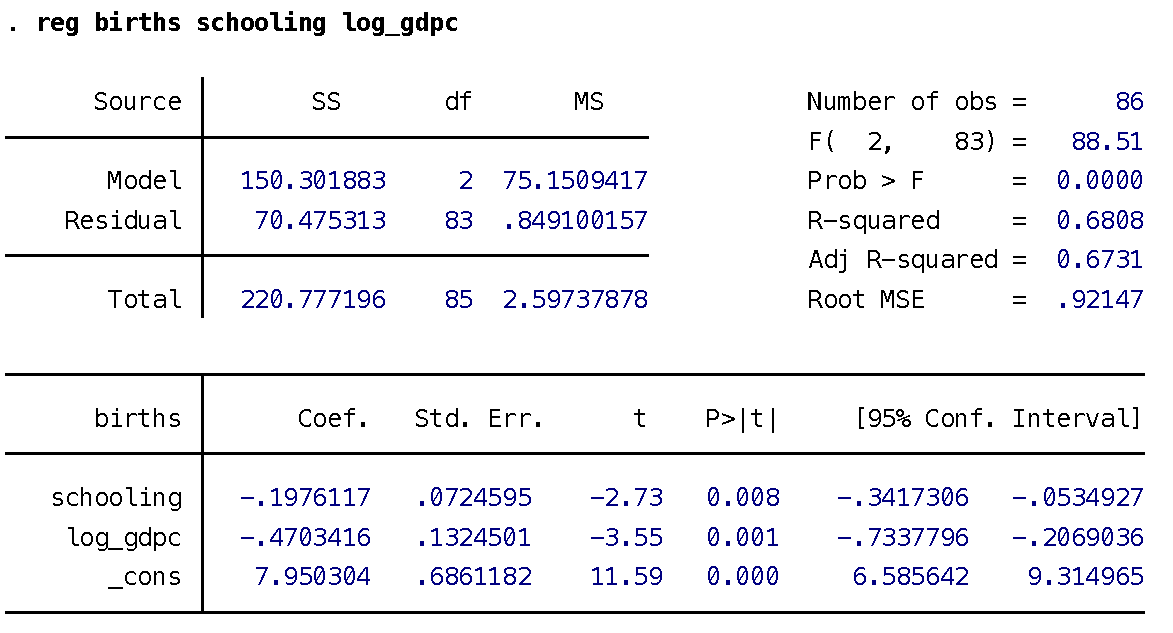
\includegraphics[scale=.45]{images/mreg-output.pdf}

	\end{frame}

	\begin{frame}[t]{Standardised coefficients}

	\code{reg births schooling log\_gdpc\red{, beta}}\\[.5em]
	
	The \code{beta} option provides \red{standardised coefficients}, which use the \textbf{standard deviation of regressors} (or predictor, i.e. the independent variables) in order to provide coefficients with comparable units:\\[.5em]

	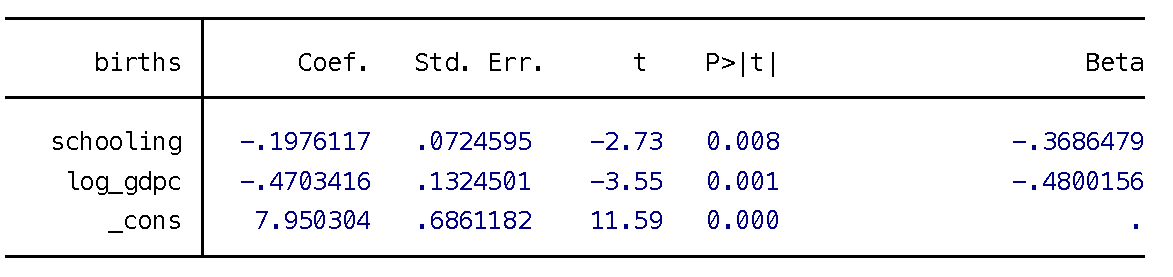
\includegraphics[scale=.45]{images/mreg-output-beta.pdf}
	
	\textit{(identical output for overall model fit omitted)}

	\end{frame}

	\begin{frame}[t]{Dummies}

	\code{reg births schooling \red{i.region}}\\[.5em]
	
	Categorical variables can be used as \red{dummies}, i.e. binary recodes of each category that are tested against a \textbf{reference category} to provide regression coefficients for net effect of that category alone:\\[.5em]
	
	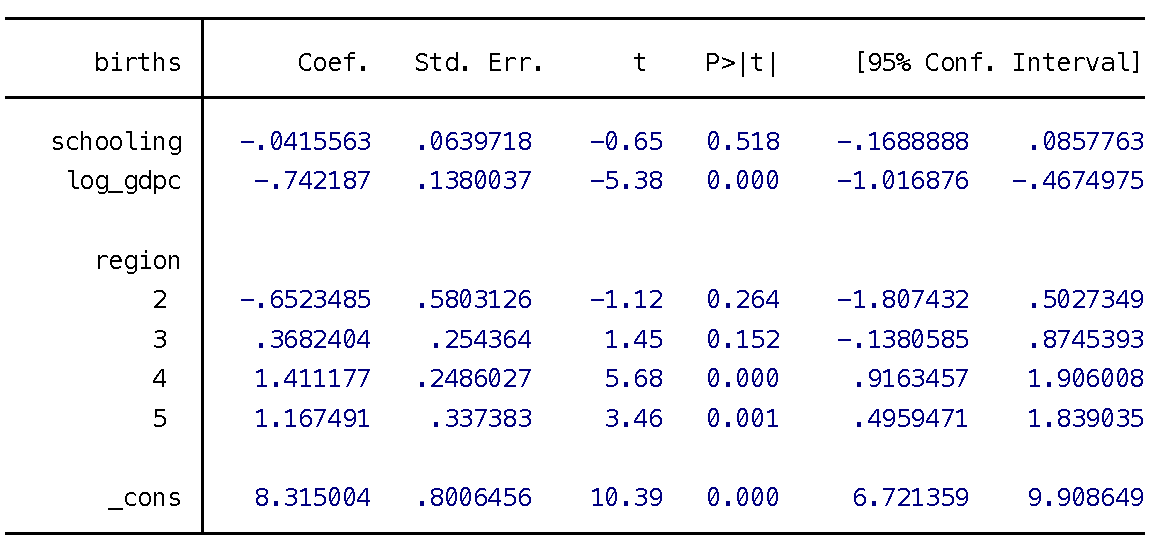
\includegraphics[scale=.45]{images/mreg-output-dummies.pdf}
	
	\textit{(identical output for overall model fit omitted)}

	\end{frame}
	
\end{document}

